
%% bare_conf.tex
%% V1.3
%% 2007/01/11
%% by Michael Shell
%% See:
%% http://www.michaelshell.org/
%% for current contact information.
%%
%% This is a skeleton file demonstrating the use of IEEEtran.cls
%% (requires IEEEtran.cls version 1.7 or later) with an IEEE conference paper.
%%
%% Support sites:
%% http://www.michaelshell.org/tex/ieeetran/
%% http://www.ctan.org/tex-archive/macros/latex/contrib/IEEEtran/
%% and
%% http://www.ieee.org/

%%*************************************************************************
%% Legal Notice:
%% This code is offered as-is without any warranty either expressed or
%% implied; without even the implied warranty of MERCHANTABILITY or
%% FITNESS FOR A PARTICULAR PURPOSE! 
%% User assumes all risk.
%% In no event shall IEEE or any contributor to this code be liable for
%% any damages or losses, including, but not limited to, incidental,
%% consequential, or any other damages, resulting from the use or misuse
%% of any information contained here.
%%
%% All comments are the opinions of their respective authors and are not
%% necessarily endorsed by the IEEE.
%%
%% This work is distributed under the LaTeX Project Public License (LPPL)
%% ( http://www.latex-project.org/ ) version 1.3, and may be freely used,
%% distributed and modified. A copy of the LPPL, version 1.3, is included
%% in the base LaTeX documentation of all distributions of LaTeX released
%% 2003/12/01 or later.
%% Retain all contribution notices and credits.
%% ** Modified files should be clearly indicated as such, including  **
%% ** renaming them and changing author support contact information. **
%%
%% File list of work: IEEEtran.cls, IEEEtran_HOWTO.pdf, bare_adv.tex,
%%                    bare_conf.tex, bare_jrnl.tex, bare_jrnl_compsoc.tex
%%*************************************************************************

% *** Authors should verify (and, if needed, correct) their LaTeX system  ***
% *** with the testflow diagnostic prior to trusting their LaTeX platform ***
% *** with production work. IEEE's font choices can trigger bugs that do  ***
% *** not appear when using other class files.                            ***
% The testflow support page is at:
% http://www.michaelshell.org/tex/testflow/


% Note that the a4paper option is mainly intended so that authors in
% countries using A4 can easily print to A4 and see how their papers will
% look in print - the typesetting of the document will not typically be
% affected with changes in paper size (but the bottom and side margins will).
% Use the testflow package mentioned above to verify correct handling of
% both paper sizes by the user's LaTeX system.
%
% Also note that the "draftcls" or "draftclsnofoot", not "draft", option
% should be used if it is desired that the figures are to be displayed in
% draft mode.
%
\documentclass[conference]{IEEEtran}
% Add the compsoc option for Computer Society conferences.
%
% If IEEEtran.cls has not been installed into the LaTeX system files,
% manually specify the path to it like:
% \documentclass[conference]{../sty/IEEEtran}





% Some very useful LaTeX packages include:
% (uncomment the ones you want to load)


% *** MISC UTILITY PACKAGES ***
%
%\usepackage{ifpdf}
% Heiko Oberdiek's ifpdf.sty is very useful if you need conditional
% compilation based on whether the output is pdf or dvi.
% usage:
% \ifpdf
%   % pdf code
% \else
%   % dvi code
% \fi
% The latest version of ifpdf.sty can be obtained from:
% http://www.ctan.org/tex-archive/macros/latex/contrib/oberdiek/
% Also, note that IEEEtran.cls V1.7 and later provides a builtin
% \ifCLASSINFOpdf conditional that works the same way.
% When switching from latex to pdflatex and vice-versa, the compiler may
% have to be run twice to clear warning/error messages.






% *** CITATION PACKAGES ***
%
%\usepackage{cite}
% cite.sty was written by Donald Arseneau
% V1.6 and later of IEEEtran pre-defines the format of the cite.sty package
% \cite{} output to follow that of IEEE. Loading the cite package will
% result in citation numbers being automatically sorted and properly
% "compressed/ranged". e.g., [1], [9], [2], [7], [5], [6] without using
% cite.sty will become [1], [2], [5]--[7], [9] using cite.sty. cite.sty's
% \cite will automatically add leading space, if needed. Use cite.sty's
% noadjust option (cite.sty V3.8 and later) if you want to turn this off.
% cite.sty is already installed on most LaTeX systems. Be sure and use
% version 4.0 (2003-05-27) and later if using hyperref.sty. cite.sty does
% not currently provide for hyperlinked citations.
% The latest version can be obtained at:
% http://www.ctan.org/tex-archive/macros/latex/contrib/cite/
% The documentation is contained in the cite.sty file itself.






% *** GRAPHICS RELATED PACKAGES ***
%
\ifCLASSINFOpdf
  \usepackage[pdftex]{graphicx}
  % declare the path(s) where your graphic files are
  % \graphicspath{{../pdf/}{../jpeg/}}
  % and their extensions so you won't have to specify these with
  % every instance of \includegraphics
  % \DeclareGraphicsExtensions{.pdf,.jpeg,.png}
\else
  % or other class option (dvipsone, dvipdf, if not using dvips). graphicx
  % will default to the driver specified in the system graphics.cfg if no
  % driver is specified.
  % \usepackage[dvips]{graphicx}
  % declare the path(s) where your graphic files are
  % \graphicspath{{../eps/}}
  % and their extensions so you won't have to specify these with
  % every instance of \includegraphics
  % \DeclareGraphicsExtensions{.eps}
\fi
% graphicx was written by David Carlisle and Sebastian Rahtz. It is
% required if you want graphics, photos, etc. graphicx.sty is already
% installed on most LaTeX systems. The latest version and documentation can
% be obtained at: 
% http://www.ctan.org/tex-archive/macros/latex/required/graphics/
% Another good source of documentation is "Using Imported Graphics in
% LaTeX2e" by Keith Reckdahl which can be found as epslatex.ps or
% epslatex.pdf at: http://www.ctan.org/tex-archive/info/
%
% latex, and pdflatex in dvi mode, support graphics in encapsulated
% postscript (.eps) format. pdflatex in pdf mode supports graphics
% in .pdf, .jpeg, .png and .mps (metapost) formats. Users should ensure
% that all non-photo figures use a vector format (.eps, .pdf, .mps) and
% not a bitmapped formats (.jpeg, .png). IEEE frowns on bitmapped formats
% which can result in "jaggedy"/blurry rendering of lines and letters as
% well as large increases in file sizes.
%
% You can find documentation about the pdfTeX application at:
% http://www.tug.org/applications/pdftex



% *** MATH PACKAGES ***
%
\usepackage[cmex10]{amsmath}
% A popular package from the American Mathematical Society that provides
% many useful and powerful commands for dealing with mathematics. If using
% it, be sure to load this package with the cmex10 option to ensure that
% only type 1 fonts will utilized at all point sizes. Without this option,
% it is possible that some math symbols, particularly those within
% footnotes, will be rendered in bitmap form which will result in a
% document that can not be IEEE Xplore compliant!
%
% Also, note that the amsmath package sets \interdisplaylinepenalty to 10000
% thus preventing page breaks from occurring within multiline equations. Use:
%\interdisplaylinepenalty=2500
% after loading amsmath to restore such page breaks as IEEEtran.cls normally
% does. amsmath.sty is already installed on most LaTeX systems. The latest
% version and documentation can be obtained at:
% http://www.ctan.org/tex-archive/macros/latex/required/amslatex/math/





% *** SPECIALIZED LIST PACKAGES ***
%
%\usepackage{algorithmic}
\usepackage{algorithm}
\usepackage{algpseudocode}
\usepackage{amssymb}	
% algorithmic.sty was written by Peter Williams and Rogerio Brito.
% This package provides an algorithmic environment fo describing algorithms.
% You can use the algorithmic environment in-text or within a figure
% environment to provide for a floating algorithm. Do NOT use the algorithm
% floating environment provided by algorithm.sty (by the same authors) or
% algorithm2e.sty (by Christophe Fiorio) as IEEE does not use dedicated
% algorithm float types and packages that provide these will not provide
% correct IEEE style captions. The latest version and documentation of
% algorithmic.sty can be obtained at:
% http://www.ctan.org/tex-archive/macros/latex/contrib/algorithms/
% There is also a support site at:
% http://algorithms.berlios.de/index.html
% Also of interest may be the (relatively newer and more customizable)
% algorithmicx.sty package by Szasz Janos:
% http://www.ctan.org/tex-archive/macros/latex/contrib/algorithmicx/




% *** ALIGNMENT PACKAGES ***
%
%\usepackage{array}
% Frank Mittelbach's and David Carlisle's array.sty patches and improves
% the standard LaTeX2e array and tabular environments to provide better
% appearance and additional user controls. As the default LaTeX2e table
% generation code is lacking to the point of almost being broken with
% respect to the quality of the end results, all users are strongly
% advised to use an enhanced (at the very least that provided by array.sty)
% set of table tools. array.sty is already installed on most systems. The
% latest version and documentation can be obtained at:
% http://www.ctan.org/tex-archive/macros/latex/required/tools/


%\usepackage{mdwmath}
%\usepackage{mdwtab}
% Also highly recommended is Mark Wooding's extremely powerful MDW tools,
% especially mdwmath.sty and mdwtab.sty which are used to format equations
% and tables, respectively. The MDWtools set is already installed on most
% LaTeX systems. The lastest version and documentation is available at:
% http://www.ctan.org/tex-archive/macros/latex/contrib/mdwtools/


% IEEEtran contains the IEEEeqnarray family of commands that can be used to
% generate multiline equations as well as matrices, tables, etc., of high
% quality.


%\usepackage{eqparbox}
% Also of notable interest is Scott Pakin's eqparbox package for creating
% (automatically sized) equal width boxes - aka "natural width parboxes".
% Available at:
% http://www.ctan.org/tex-archive/macros/latex/contrib/eqparbox/





% *** SUBFIGURE PACKAGES ***
%\usepackage[tight,footnotesize]{subfigure}
% subfigure.sty was written by Steven Douglas Cochran. This package makes it
% easy to put subfigures in your figures. e.g., "Figure 1a and 1b". For IEEE
% work, it is a good idea to load it with the tight package option to reduce
% the amount of white space around the subfigures. subfigure.sty is already
% installed on most LaTeX systems. The latest version and documentation can
% be obtained at:
% http://www.ctan.org/tex-archive/obsolete/macros/latex/contrib/subfigure/
% subfigure.sty has been superceeded by subfig.sty.



%\usepackage[caption=false]{caption}
%\usepackage[font=footnotesize]{subfig}
% subfig.sty, also written by Steven Douglas Cochran, is the modern
% replacement for subfigure.sty. However, subfig.sty requires and
% automatically loads Axel Sommerfeldt's caption.sty which will override
% IEEEtran.cls handling of captions and this will result in nonIEEE style
% figure/table captions. To prevent this problem, be sure and preload
% caption.sty with its "caption=false" package option. This is will preserve
% IEEEtran.cls handing of captions. Version 1.3 (2005/06/28) and later 
% (recommended due to many improvements over 1.2) of subfig.sty supports
% the caption=false option directly:
%\usepackage[caption=false,font=footnotesize]{subfig}
%
% The latest version and documentation can be obtained at:
% http://www.ctan.org/tex-archive/macros/latex/contrib/subfig/
% The latest version and documentation of caption.sty can be obtained at:
% http://www.ctan.org/tex-archive/macros/latex/contrib/caption/




% *** FLOAT PACKAGES ***
%
%\usepackage{fixltx2e}
% fixltx2e, the successor to the earlier fix2col.sty, was written by
% Frank Mittelbach and David Carlisle. This package corrects a few problems
% in the LaTeX2e kernel, the most notable of which is that in current
% LaTeX2e releases, the ordering of single and double column floats is not
% guaranteed to be preserved. Thus, an unpatched LaTeX2e can allow a
% single column figure to be placed prior to an earlier double column
% figure. The latest version and documentation can be found at:
% http://www.ctan.org/tex-archive/macros/latex/base/



%\usepackage{stfloats}
% stfloats.sty was written by Sigitas Tolusis. This package gives LaTeX2e
% the ability to do double column floats at the bottom of the page as well
% as the top. (e.g., "\begin{figure*}[!b]" is not normally possible in
% LaTeX2e). It also provides a command:
%\fnbelowfloat
% to enable the placement of footnotes below bottom floats (the standard
% LaTeX2e kernel puts them above bottom floats). This is an invasive package
% which rewrites many portions of the LaTeX2e float routines. It may not work
% with other packages that modify the LaTeX2e float routines. The latest
% version and documentation can be obtained at:
% http://www.ctan.org/tex-archive/macros/latex/contrib/sttools/
% Documentation is contained in the stfloats.sty comments as well as in the
% presfull.pdf file. Do not use the stfloats baselinefloat ability as IEEE
% does not allow \baselineskip to stretch. Authors submitting work to the
% IEEE should note that IEEE rarely uses double column equations and
% that authors should try to avoid such use. Do not be tempted to use the
% cuted.sty or midfloat.sty packages (also by Sigitas Tolusis) as IEEE does
% not format its papers in such ways.





% *** PDF, URL AND HYPERLINK PACKAGES ***
%
%\usepackage{url}
% url.sty was written by Donald Arseneau. It provides better support for
% handling and breaking URLs. url.sty is already installed on most LaTeX
% systems. The latest version can be obtained at:
% http://www.ctan.org/tex-archive/macros/latex/contrib/misc/
% Read the url.sty source comments for usage information. Basically,
% \url{my_url_here}.





% *** Do not adjust lengths that control margins, column widths, etc. ***
% *** Do not use packages that alter fonts (such as pslatex).         ***
% There should be no need to do such things with IEEEtran.cls V1.6 and later.
% (Unless specifically asked to do so by the journal or conference you plan
% to submit to, of course. )


% correct bad hyphenation here
\hyphenation{op-tical net-works semi-conduc-tor}

% suppress indentation at beginning of paragraphs
\usepackage[parfill]{parskip}

\begin{document}
%
% paper title
% can use linebreaks \\ within to get better formatting as desired
\title{Melon Protocol Specification}


% author names and affiliations
% use a multiple column layout for up to three different
% affiliations
\author{\IEEEauthorblockN{Melonport AG}
\IEEEauthorblockA{team@melonport.com}}

% conference papers do not typically use \thanks and this command
% is locked out in conference mode. If really needed, such as for
% the acknowledgment of grants, issue a \IEEEoverridecommandlockouts
% after \documentclass

% for over three affiliations, or if they all won't fit within the width
% of the page, use this alternative format:
% 
%\author{\IEEEauthorblockN{Michael Shell\IEEEauthorrefmark{1},
%Homer Simpson\IEEEauthorrefmark{2},
%James Kirk\IEEEauthorrefmark{3}, 
%Montgomery Scott\IEEEauthorrefmark{3} and
%Eldon Tyrell\IEEEauthorrefmark{4}}
%\IEEEauthorblockA{\IEEEauthorrefmark{1}School of Electrical and Computer Engineering\\
%Georgia Institute of Technology,
%Atlanta, Georgia 30332--0250\\ Email: see http://www.michaelshell.org/contact.html}
%\IEEEauthorblockA{\IEEEauthorrefmark{2}Twentieth Century Fox, Springfield, USA\\
%Email: homer@thesimpsons.com}
%\IEEEauthorblockA{\IEEEauthorrefmark{3}Starfleet Academy, San Francisco, California 96678-2391\\
%Telephone: (800) 555--1212, Fax: (888) 555--1212}
%\IEEEauthorblockA{\IEEEauthorrefmark{4}Tyrell Inc., 123 Replicant Street, Los Angeles, California 90210--4321}}

% use for special paper notices
%\IEEEspecialpapernotice{(Invited Paper)}

% make the title area
\maketitle

\begin{abstract}
%\boldmath
The abstract goes here.
\end{abstract}
% IEEEtran.cls defaults to using nonbold math in the Abstract.
% This preserves the distinction between vectors and scalars. However,
% if the conference you are submitting to favors bold math in the abstract,
% then you can use LaTeX's standard command \boldmath at the very start
% of the abstract to achieve this. Many IEEE journals/conferences frown on
% math in the abstract anyway.

% no keywords




% For peer review papers, you can put extra information on the cover
% page as needed:
% \ifCLASSOPTIONpeerreview
% \begin{center} \bfseries EDICS Category: 3-BBND \end{center}
% \fi
%
% For peerreview papers, this IEEEtran command inserts a page break and
% creates the second title. It will be ignored for other modes.
\IEEEpeerreviewmaketitle



\section{Introduction}

Fund administration consists of four parts. Fund Custodian, Fund Accountant, KYC/AML and Risk Management. In the following paper we will describe how fund administration can be implemented using smart contracts.

\section{Background}

\subsection{Custodian}

\subsection{Decentralized Execution}

\subsubsection{Assets}

An example for such computer code is known as the ERC20 standard. Essentially a small ($<100$ lines of code) piece of software implementing a bitcoin-like cryptocurrency.

\subsubsection{Exchanges}

Another example are exchanges. Given above concept one now can implement computer code one how exchange of above assets can be facilitated in a decentralised way.

\subsubsection{Investment Funds}

Using the concept that smart contracts can be custodian of assets. Once a smart contract holds assets there needs the be custom functions built into the smart-contract in order to spend those assets again. Lack of such function means that assets are forever lost.

we can now build smart contracts that act as fully functional investment funds.

To manage their holdings these investment funds use decentralised exchanges to buy and sell assets.


\section{Investment Funds Design}

\subsection{Governance}

\begin{figure*}[ht!]
	\centering
	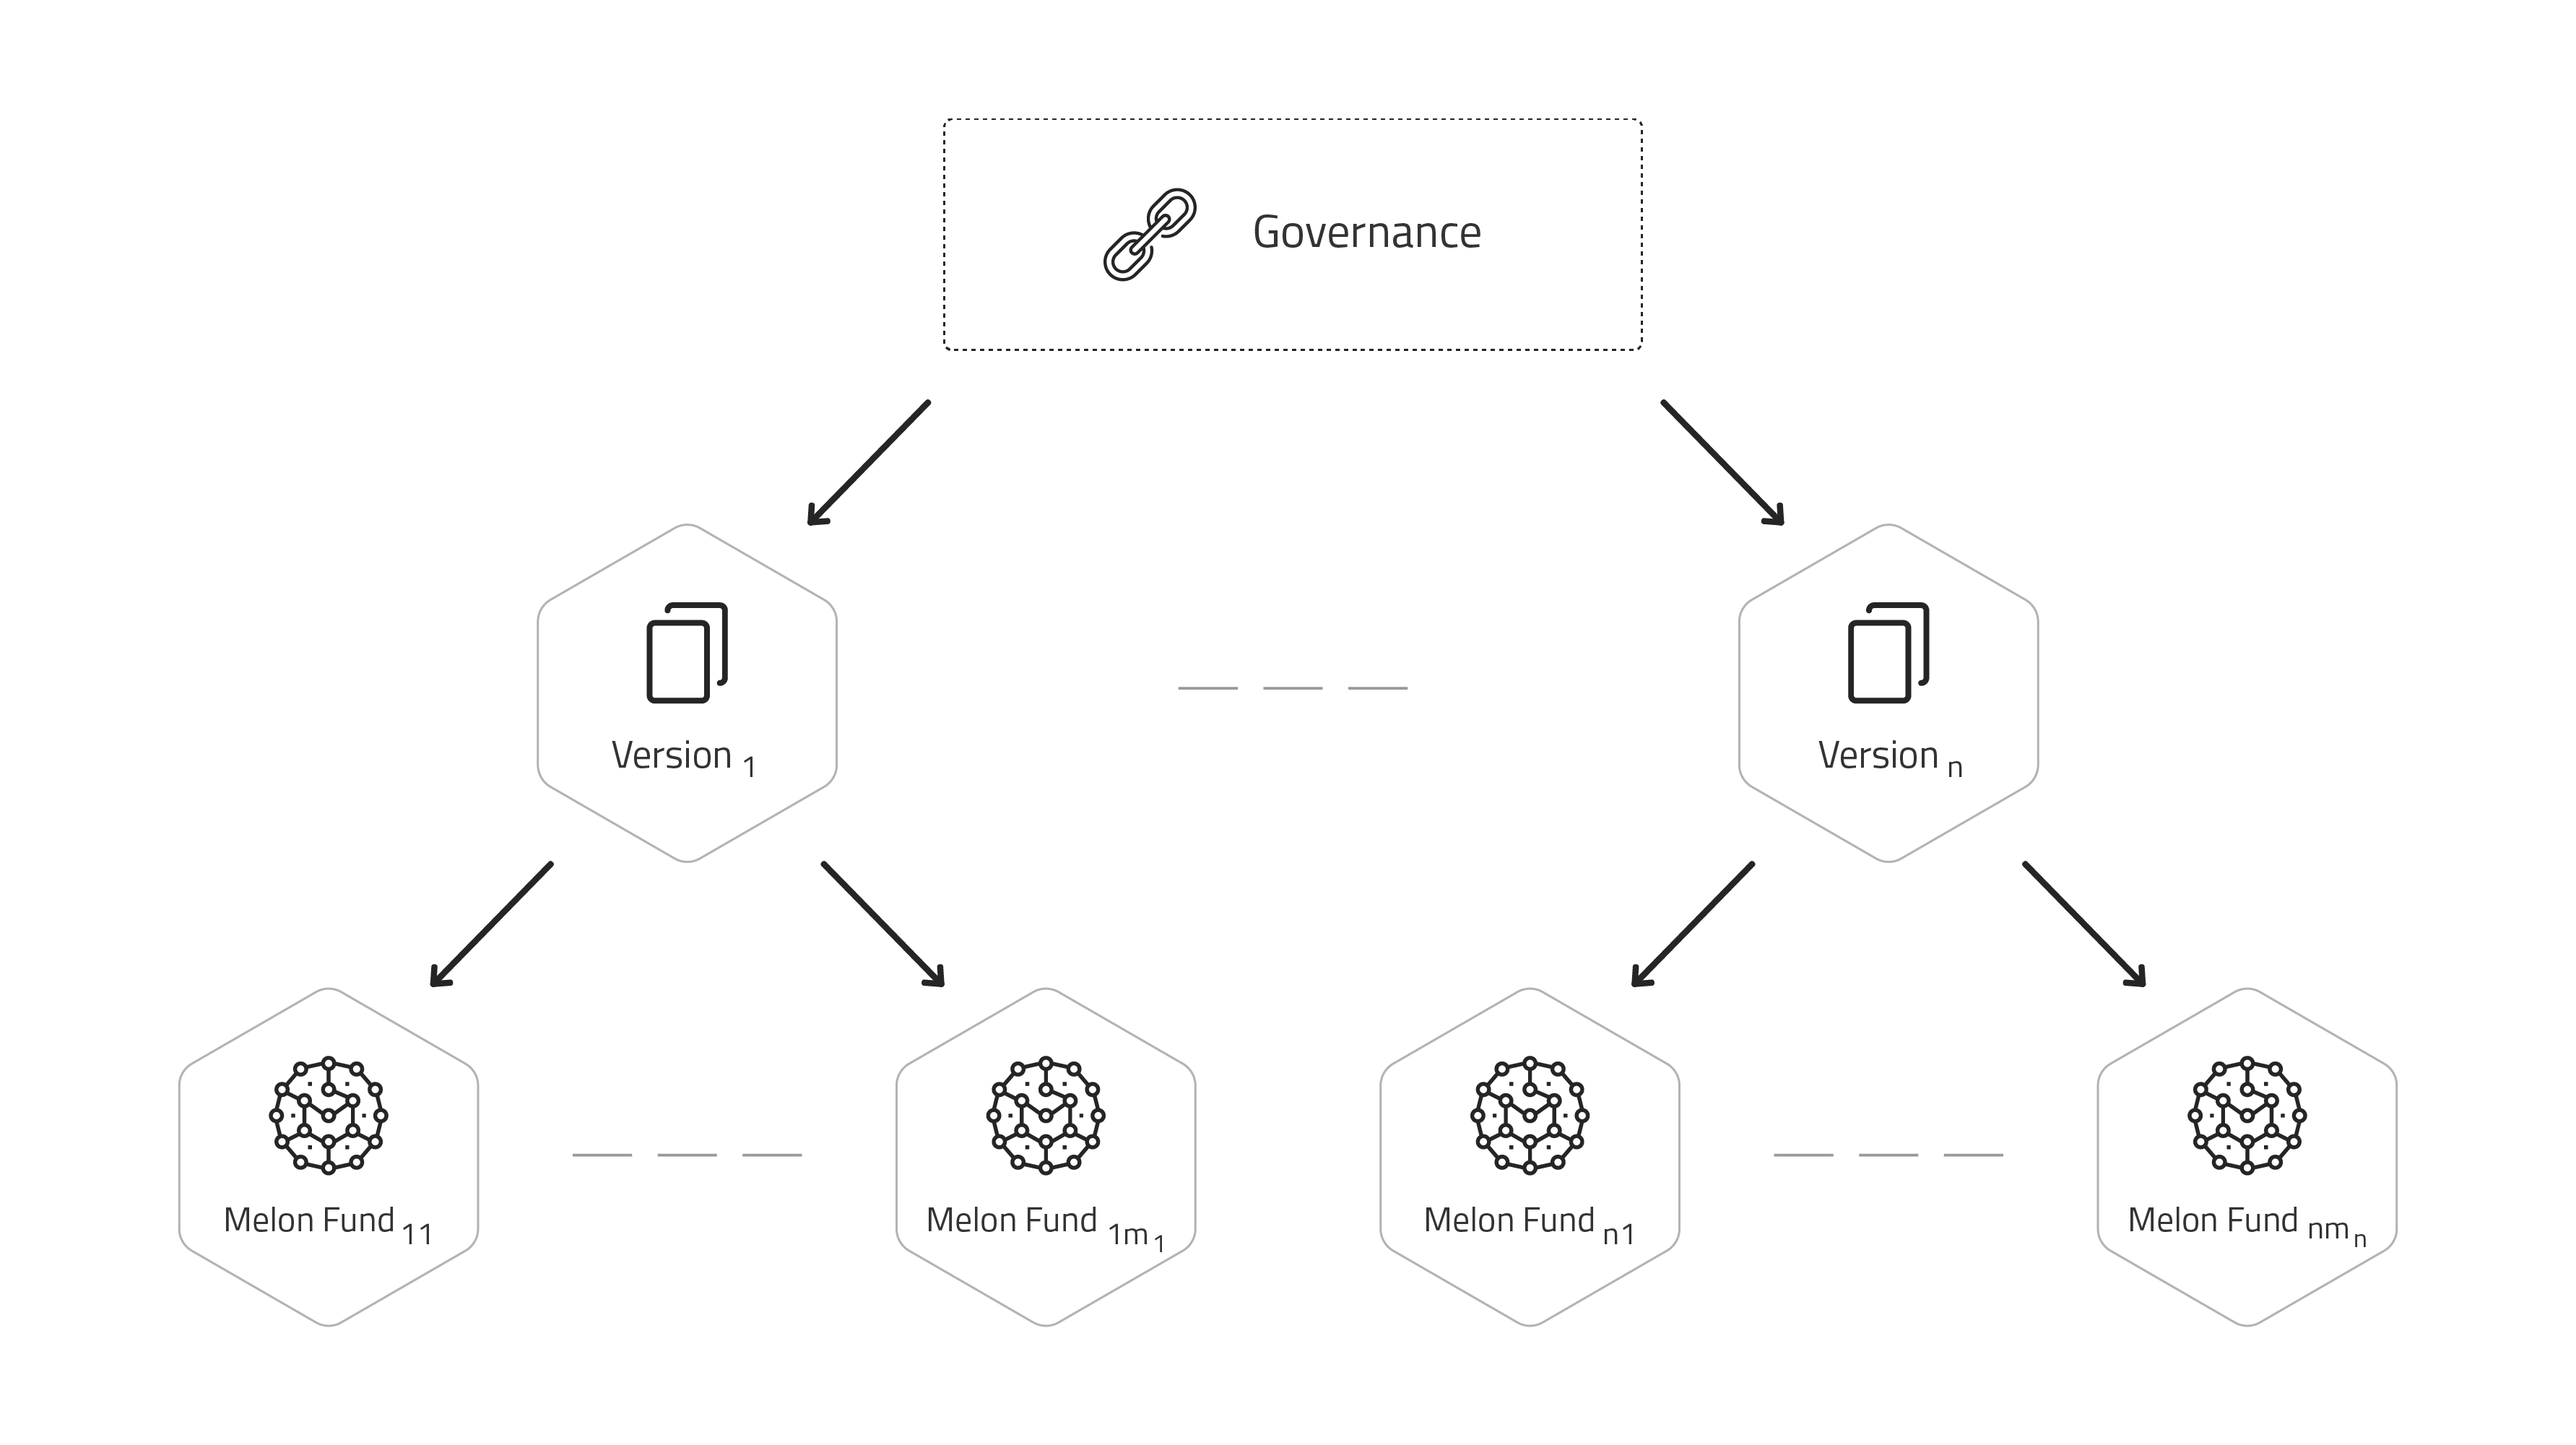
\includegraphics[width=135mm]{images/governance.png}
	\caption{Protocol governance linked to versions linked to Melon funds\label{fig:governance}}
\end{figure*}

The main functionality of the Governance contract is to add new protocol versions such as this Version contract and to shut down existing versions once they become obsolete.

Adding a \textit{new protocol version} is done by anyone proposing a version to be added and is executed once authority consensus has been established.

Shutting down an existing protocol version is done by anyone proposing a version to be shut down and is executed once authority consensus has been established.

Shutting down a version disables the ability to setup new funds using this version and enables anyone to shut down any existing funds of this version.

\subsection{Investment Fund}\label{fund}

Melon fund as a smart contract that acts as the custodian and accountant. Broadly speaking a Melon fund should be capable of accepting/executing subscription and redemption requests, make orders on an exchange, take orders on an exchange and
receiving management and performance rewards.

A Melon fund is created by triggering a Solidity function in the version contract.

\subsection{Modules}

\begin{figure*}[ht!]
	\centering
	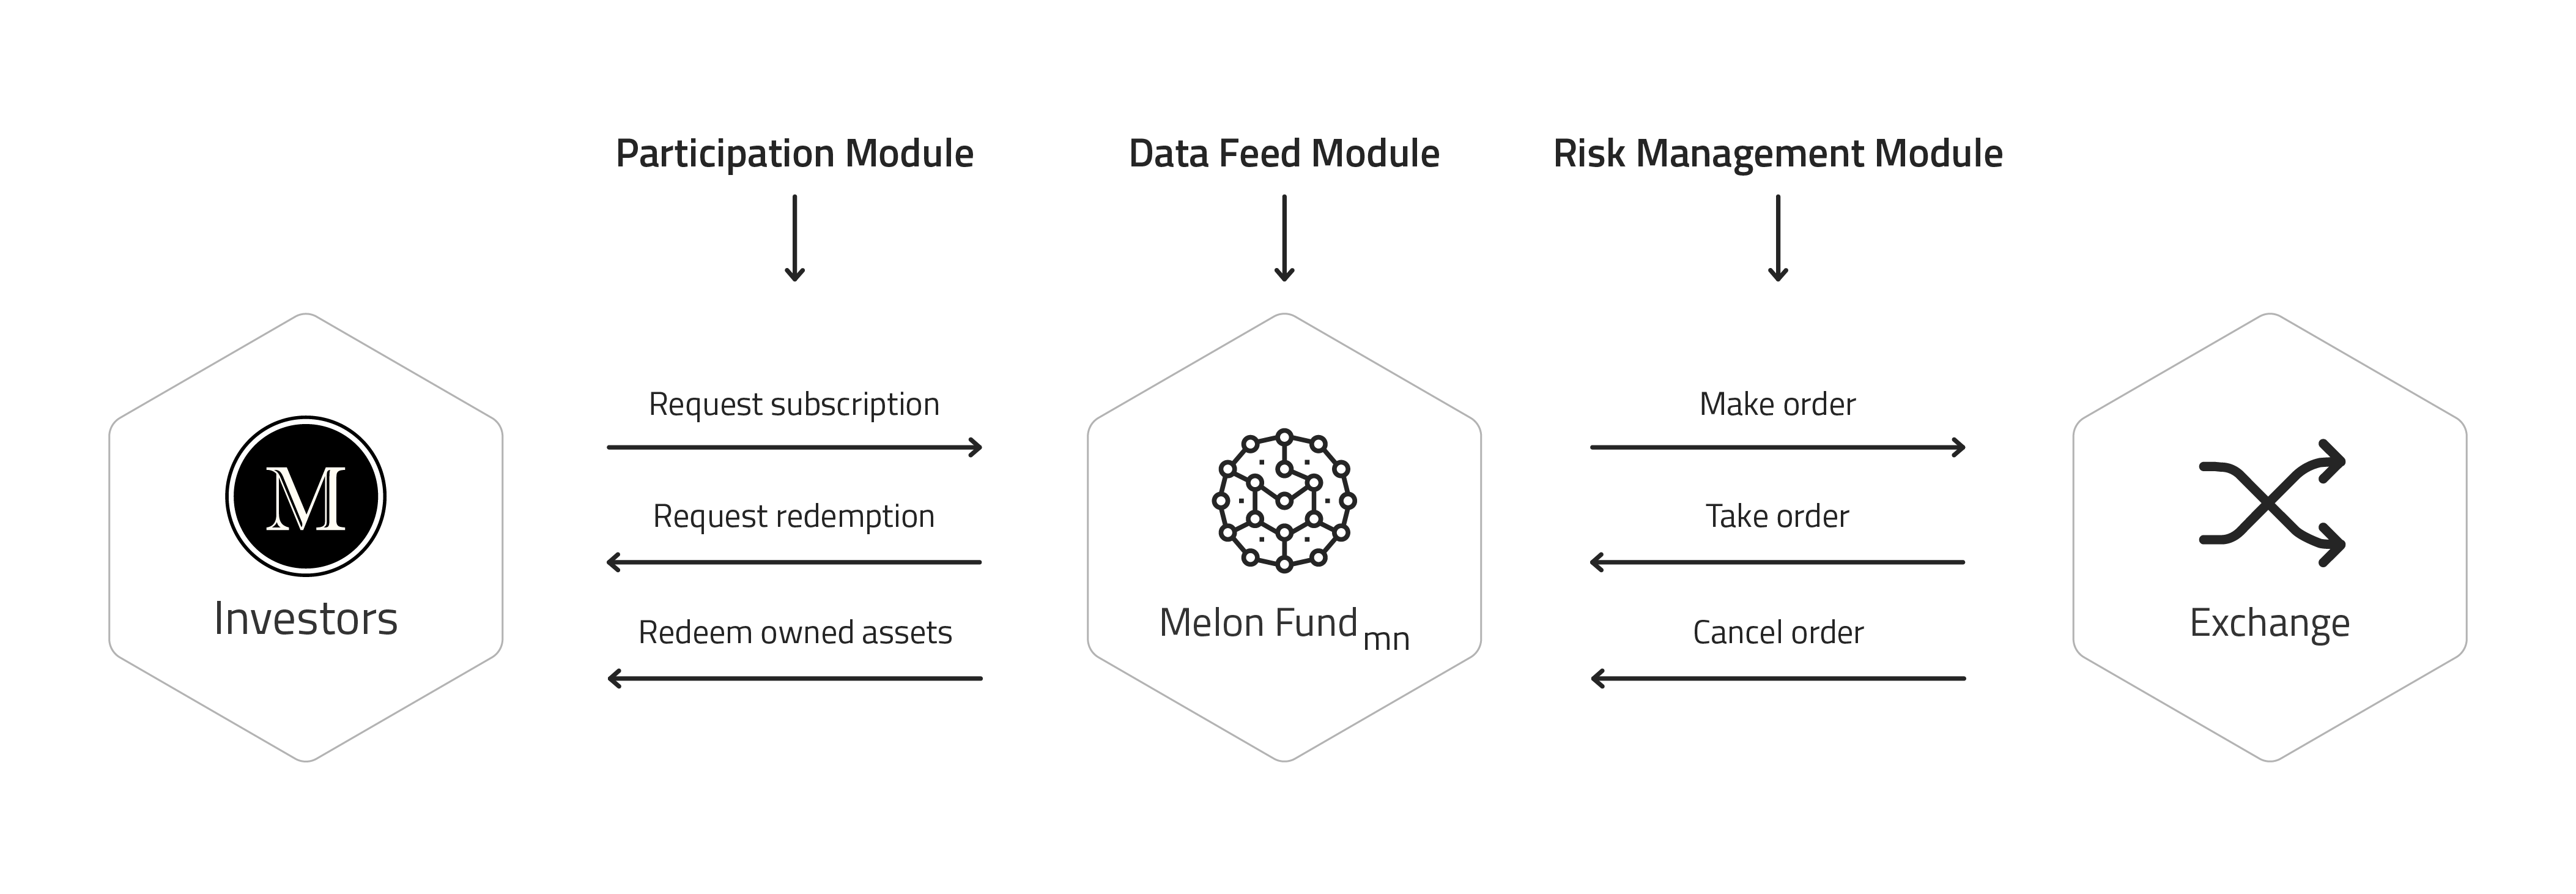
\includegraphics[width=135mm]{images/fund.png}
	\caption{Melon fund interaction with Melon modules\label{fig:fund}}
\end{figure*}

Functionality outside the core Fund logic is provided by \textit{Melon modules}. These modules interact with the Fund in a standardized way, depending on their type.
This enables modules to be interchangeable within their class, such that two modules of the same class may fill the same \textit{role}, albeit with differing logic, parameters or other characteristics.

Modules, operating outside the core of the protocol, may be built by third parties without the permission of Melon protocol maintainers.
\textit{Module builders} are incentivised to create and maintain modules through an inflation mechanism built into the protocol. 
They are rewarded with Melon tokens based on some usage characteristics for their module.

Melon has six different module classes:

\begin{itemize}
  \item Exchange Adapters
  \item Rewards
  \item Participation
  \item Risk Management
  \item Asset registrar
  \item Data feed
\end{itemize}

% TODO: maybe just label the above entries with their category?
These classes can be categorized into three subsets:

\begin{itemize}
  \item Libraries
  \item Boolean functions
  \item Infrastructure
\end{itemize}

\section{Specifications}

\subsection{Asset Registrar}

Asset registrar module is intended for registering assets and information associated with them on-chain. Subsequent modules check if an asset is registered in the Asset registration before performing different operations. Registration can be done via the register function that takes the following parameters:

\begin{center}
	\footnotesize
	\begin{tabular}{ | p{2.7cm} | p{0.8cm} | p{4cm} | }
		\hline
		Name & Data Type & Description \\ \hline
		ofAsset & address & A human readable name of the fund \\ \hline
		name & string & Human-readable name of the Asset as in ERC223 token standard \\ \hline
		symbol & string & Human-readable symbol of the Asset as in ERC223 token standard \\ \hline
		decimal & uint & Number of decimals for precision \\ \hline
		url & string & for extended information of the assetn \\ \hline
		ipfsHash & bytes32 & Same as url but for ipfs \\ \hline
		chainId & bytes32 & Chain where the asset resides \\ \hline
		breakIn & address & Address of break in contract on destination chain \\ \hline
		breakOut & address & Address of break out contract on this chain \\ \hline
	\end{tabular}
\end{center}

Since storage on-chain is expensive, a url and / or an ipfsHash of the document containing asset information is stored. An ipfsHash is although preferred to ensure data integrity.

Due to gas limit contraints, the constant field named $maxAssets$ defines the maximum number of assets that can be registered. This number is calculated by checking the maximum number of registered assets $redeemOwnedAssets$ function supports. This specific function is chosen because it is the most gas intensive operation that grows linearly with number of registered assets. 


$maxAssets$: ($blockGasLimit$ - $rGas_1$) /  $\Delta_{(rGas_n, rGas_{n-1}]}$ where $rGas_n$ is the worst-case gas consumed by redeemOwnedAssets function for 'n' registered assets.

\subsection{Data Feed}  \label{component:data-feed}

Data feeds are instances of smart contracts that route external data which include asset prices into smart contracts. These inputs could be staked and validated on-chain in order to prevent incorrect / manipulative inputs.  

Data feed uses update to periodically update prices of all the assets in one pass. Historic updates are also stored for reference purposes.

$getReferencePrice$ can be used to query the price of any given asset in reference to another asset. As of now, It is necessary that either of the assets needs to be the reference asset ($quoteAsset$) which is set during contract creation. Following the analogy of currency pair, it takes the addresses of the base and quote assets as the input parameters. The quote asset is used as a reference to return the relative value of the base asset.

If the quote asset is just the reference asset, the latest updated price of the base asset from the data history is returned. If not, $getInvertedPrice$ is called which returns the price based on the formula of $getDecimals(baseAsset)$  * $getDecimals(quoteAsset))$ / $latestPrice(baseAsset)$. It basically returns the price of reference asset relative to the base asset. It also ensures input and quote assets are compatible in terms of precision (decimals).

$getOrderPrice$ takes the inputs of address of base asset, sellQuantity and buyQuantity. It returns the price of the order based on these inputs using $buyQuantity * (10 ** uint(getDecimals(ofBase))) / (sellQuantity)$. 

\begin{algorithm}
	\caption{Update algorithm}
	\label{update}
	\begin{algorithmic}[1] % The number tells where the line numbering should start
		\Procedure{update}{$assets,prices$} \Comment{Update asset prices}
		\State $i\gets nextUpdateId$
		\For{$j=0$; $j < assets.length$; $j \gets j+1$}
		\State $dataHistory[i][assets[j]] \gets prices[j]$ \Comment{To keep track of historial price updates}
		\EndFor\label{euclidendwhile}
		\State $nextUpdateId \gets nextUpdateId + 1$
		\EndProcedure
	\end{algorithmic}
\end{algorithm}

\subsection{Accounting} \label{component:accounting}

Accounting keeps track of gav (gross asset value) of the fund. It is currently not a separate module but rather a part of the fund contract. Gross asset value is calculated by:


$gav = \sum_{k=1}^{n} assetHoldings(a_k) * assetPrice(a_k)$


where n is the number of registered assets in the asset registrar module. $assetHoldings(a_k)$  is the quantity of assets of type k held by the fund and $assetPrice(a_k)$ is the price of the asset of type k which is obtained from the datafeed module.


\subsection{Rewards}

There are two kinds of rewards associated with a fund: \textit{performance} and \textit{management} rewards.
Both are meant as forms of compenesation for the fund manager. Management reward is proportional to the duration of management for a fund.
Performance reward, on the other hand is solely based on the performance of the fund.

\subsubsection{Calculation}

Performance rewards are calculated by the formula $investmentProfits * performanceRewardRate$.
Here, $performanceRewardRate$ is expressed as a percentage, and $investmentProfits$ refers to the positive change in share price of the fund from the last high-water mark (excluding any unclaimed performance rewards) multiplied by the total number of shares.

\textit{High-water mark} refers to the maximum share price within a given interval.
Using this, we ensure that the fund manager is neither rewarded for poor performance, nor rewarded multiple times for the same performance.
The high-water mark is updated each time the manager performs rewards redemption (conversion into shares).

Management rewards are calculated by the formula $((timeDifference * gav) / 1 year) * managementRewardRate$.
Here, $managementRewardRate$ is expressed as a percentage. This is the percentage of the fund's gross asset value extracted through management fees on a yearly basis.

\subsubsection{Redemption}

As might be expected, performance rewards are only paid out in the case of the fund's share price increasing.
Therefore, a decrease in performance will not \textit{cost} the manager any money, in the form of a negative performance reward.

In contrast to performance rewards, management rewards are paid out based on duration of management, irrespective of fund performance.

Redemption of both reward types occurs simultaneously, and can be triggered at the manager's discretion.
The rewards are given to the manager in the form of an allocation of the fund's shares.
That is, at redemption time, the manager receives newly-minted shares of their own fund.
Thus, the shareholders pay their fees in the form of share inflation, rather than directly subtracting from their balance of any particular token.

\subsection{Participation}

Participation module specifies rules for whitelisting investors. It comprises of two boolean functions $isSubscriptionPermitted$ and $isRedemptionPermitted$ which enforce rules to check if a particular address is allowed to invest and redeem from the fund. The functions $attestForIdentity$ and $removeAttestion$ both of which take a single parameter of the participant address can be used to add or remove  the participant address from the whitelist respectively. 

\subsection{Exchange Adapter}

The \textit{exchange adapter} is an adapter between the Melon protocol and decentralized exchanges such as OasisDex, Kyber, or Bancor.

The exchange adapter contract is designed to be used as a proxy for the exchange itself, adapting the exchange's methods to be in line with the interface that the fund expects.
The adapter is also pre-deployed, and is chosen when a manager initially sets up a fund.

This contract differs from some of the others in that its methods are called \textit{in the context of the fund}, using $delegateCall$.
By doing this, the fund directly interacts with the exchange, albeit via adapted methods present on the adapter.
This ultimately allows the fund contract's internal order management code to remain identical \textit{across all funds}, while retaining the ability for fund managers to interact with their preferred exchanges.

The exact implementation details of the adapter methods depend on the exchange we are interfacing with, but there are three primary functions.

The first, $makeOrder$ can be used to make an order on the given exchange. It takes the following input parameters:
\begin{center}
	\footnotesize
	\begin{tabular}{ | p{2.7cm} | p{0.8cm} | p{4cm} | }
		\hline
		Name & Data Type & Description \\ \hline
		onExchange & address & Address of the exchange \\ \hline
		sellAsset & address &  Reference price obtained through DataFeed contract \\ \hline
		buyAsset & address & Asset (as registered in Asset registrar) to be bought \\ \hline
		sellQuantity & uint & Quantity of sellAsset to be sold \\ \hline
		buyQuantity & uint & Quantity of buyAsset to be bought \\ \hline
	\end{tabular}
\end{center}

Second, $takeOrder$ can be used to take a specific order on the given exchange. It takes the following input parameters:
\begin{center}
	\footnotesize
	\begin{tabular}{ | p{2.7cm} | p{0.8cm} | p{4cm} | }
		\hline
		Name & Data Type & Description \\ \hline
		onExchange & address & Address of the exchange \\ \hline
		id & uint & Order id \\ \hline
		quantity & uint & Quantity of order to be executed (For partial taking) \\ \hline
	\end{tabular}
\end{center}

Finally, $cancelOrder$ can be used to cancel a specific order. It takes the following input parameters:
\begin{center}
	\footnotesize
	\begin{tabular}{ | p{2.7cm} | p{0.8cm} | p{4cm} | }
		\hline
		Name & Data Type & Description \\ \hline
		onExchange & address & Address of the exchange \\ \hline
		id & uint & Order id \\ \hline
	\end{tabular}
\end{center}

\subsection{Risk Management}

Risk management module primarily comprises of two boolean functions $isMakePermitted$ and $isTakePermitted$ both of which take input the following parameters:

\begin{center}
	\footnotesize
	\begin{tabular}{ | p{2.7cm} | p{0.8cm} | p{4cm} | }
		\hline
		Name & Data Type & Description \\ \hline
		orderPrice & uint & Price of Order \\ \hline
		referencePrice & uint &  Reference price obtained through DataFeed contract \\ \hline
		sellAsset & address & Asset (as registered in Asset registrar) to be sold \\ \hline
		buyAsset & address & Asset (as registered in Asset registrar) to be bought \\ \hline
		sellQuantity & uint & Quantity of sellAsset to be sold \\ \hline
		buyQuantity & uint & Quantity of buyAsset to be bought \\ \hline
	\end{tabular}
\end{center}

Custom logic can be defined based on the input parameters that enforces the behaviour of those two boolean functions. (Example: return true if $orderPrice >= referencePrice$). 

Our simple flavor of risk management module is called RMMakeOrders. It checks whether the orderPrice falls within the maximum allowed deviation relative to the reference price.
RMMakeOrders evaluates $orderPrice <= referencePrice - (riskLevel  * referencePrice) / riskDivisor$ and disallows the make or take order if it is true.
$riskLevel$ is the magnitude of deviation allowed from reference price. 

The intuition behind it is that the order price should always be higher than or close to the reference price.
Order price is directly proportional to the buyQuantity and inversely proportional to the sellQuantity. It is always beneficial to have the buyQuantity as high as possible.

\subsection{Version}

The Version contract maps one-to-one with a protocol version, meaning that each deployment of the protocol contains a single Version contract.

The purpose of the deployed Version is to index Funds in each protocol version, and to allow managers to set up and shut down their Funds.
Indeed, Funds can \textit{only} be created through calling $setupFund$ on a particular Version contract (\ref{interaction:setup-fund}).
Thus, with each particular Version, the interface and initial template of each new fund is identical.
Likewise, Funds can be shut down with the manager calling $shutDownFund$ through the Version with which the Fund was deployed.

This method of deploying Funds lends itself well to Governance; old Versions can be deprecated to eliminate bugs, or new Versions introduced to add features.
Adding a Version starts with a proposal for a new Version, and is executed when authority consensus is established.
This process is performed by the Governance contract, and is described in \ref{component:governance}.
Similarly, a Version contract is deprecated when the Governance contract calls $shutDown$ on the Version, again requiring authority consensus.
This prevents new Funds from being created by this Version, and allows anyone to shut down Funds created through it.

The parameters required for creating a new Version are as follows:

\begin{center}
	\footnotesize
	\begin{tabular}{ | p{2cm} | p{1.2cm} | p{4cm} | }
		\hline
		Name & Data Type & Description \\ \hline
		versionNumber & string & Unique identifier for this protocol version \\ \hline
		ofGovernance & address & The Governance contract responsible for this Version \\ \hline
		ofMelonAsset & address & The Melon token for the current blockchain  \\ \hline
	\end{tabular}
\end{center}


\subsection{Governance} \label{component:governance}

Governance uses \textit{ds-group} module to require and establish consensus of authorities for the operations of adding and shutting down versions. Governance contract is first created by specifying the following parameters:

\begin{center}
	\footnotesize
	\begin{tabular}{ | p{2cm} | p{1.2cm} | p{4cm} | }
		\hline
		Name & Data Type & Description \\ \hline
		ofAuthorities & address[] & Array of addresses of authorities \\ \hline
		ofQuorum & uint & Minimum number of signatures from authorities required for proposal to pass by \\ \hline
		ofWindow & uint & Time limit for proposal validity \\ \hline
	\end{tabular}
\end{center}


$proposeVersion$ can be used by an authority to propose a new version address.

$approveVersion$ can be used by an authority other than the proposer to specify their endorsement for the new version proposal.  Number of confirmations is incremented.

$triggerVersion$ checks if the number of confirmations for that particular version proposal satisfies the quorum condition and adds the proposed version to the version list. 

Shutting down a version follows a similar flow with the methods $proposeShutdown$, $approveShutdown$ and $triggerShutdown$ instead.

\section{Interactions}

This section describes how the three main agents of the Melon protocol interact with each other.

The three main agents being: Investor, Manager, Module Operator.

\subsection{Operator runs Asset registrar}

An asset registrar tracks the universe of assets available for management, and information about each asset.
The operator is responsible for keeping the registry in check, which may include adding and removing assets.

If an operator desires to register an asset, he must call the $register$ function with information about the asset including, but not limited to, its contract address, name, and ticker symbol.
An operator may de-register an asset simply by calling $remove$ with the asset's contract address.

\subsection{Operator runs Data feed}

A Data feed module requires regular updates from an operator, which act according to the algorithm described in \ref{component:data-feed}.
The data injected into the feed is used within the fund for accounting purposes, such as calculating the price of shares.
The $update$ function receives the following inputs:

\begin{center}
		\footnotesize
		\begin{tabular}{ | p{2.7cm} | p{0.8cm} | p{4cm} | }
		\hline
		Name & Data Type & Description \\ \hline
        ofAssets & address[] & Array of asset addresses \\ \hline
        newPrices & uint[] & Array of asset prices, in terms of reference asset \\ \hline
		\end{tabular}
\end{center}

It is the operator's responsibility to call $update$ at the interval defined at data feed setup.

\subsection{Operator runs Participation module}

An operator can use $attestForIdentity$ and $removeAttestation$ to achieve the vanilla functionality of whitelisting and removing from whitelist an investor. They may also define additional functionality, e.g. requiring the subscribing participant to be in a special whitelist status in case the subscription request is for more than 'n' number of shares.

\subsection{Operator runs Risk management module}

An operator can define custom logic for risk management based on order and reference prices. It can also include dynamic data inputs. E.g. Operator can add checks on orderPrice by aggregating the referencePrices from different exchanges. This can be done by inputting price data from different exchanges on-chain periodically preferrably through a custom data feed module.

\subsection{Manager sets up a new Melon fund}	\label{interaction:setup-fund}

A new Melon fund can be setup by specifying the following parameters via setupFund function of the version contract:

\begin{center}
		\footnotesize
		\begin{tabular}{ | p{2.7cm} | p{0.8cm} | p{4cm} | }
		\hline
		Name & Data Type & Description \\ \hline
		name & string & A human readable name of the fund \\ \hline
		referenceAsset & address & Asset against which performance reward is measured against \\ \hline
		managementRewardRate & uint	& Reward rate in referenceAsset per delta improvement \\ \hline
		performanceRewardRate & uint & Reward rate in referenceAsset per managed seconds \\ \hline
		participation & address	& Participation module \\ \hline
		riskMgmt & address & Risk management module \\ \hline
		sphere & address & Sphere module \\ \hline
		\end{tabular}
\end{center}

\subsection{Participant invests in a Melon fund} \label{interaction:invest}

A participant starts to invest in a fund $F$ by first creating a subscription request $R$.

Parameters to be specified are:

\begin{center}
		\footnotesize
		\begin{tabular}{ | p{2.7cm} | p{1.2cm} | p{4cm} | }
		\hline
		Name & Data Type & Description \\ \hline
		giveQuantity & uint & Quantity of Melon tokens to invest \\ \hline
		shareQuantity & uint & Quantity of fund shares to receive \\ \hline
		incentiveQuantity & uint & Quantity of Melon tokens to award the entity executing the request \\ \hline
	\end{tabular}
\end{center}

Properties of $R$ are checked against restriction rules specified in the participation module $P$ by the boolean function $isSubscriptionPermitted$ (e.g checking whether a participant has an attested Uport identity).

$R$ is then executed by some entity calling $executeRequest$ after certain conditions are satisfied, described immediately below in \ref{delayed-requests}.

\subsubsection{Delayed requests} \label{delayed-requests}

The nature of the blockchain means that data can only be delivered in intervals, the minimum interval being a single blocktime.
Because of this, smart contracts are only able to receive and operate on data in intervals as well.
Thus, an agent $A$ with access to real time data could interact with a smart contract $C$ between data delivery intervals, and have an information advantage over the contract.

To describe the vulnerability of this model in terms of a Melon fund, let us assume that the share price $S$ is defined as in \ref{component:accounting}, and that $S$ is calculated at regular intervals $I$, such that $I$ is some number of blocktimes.

We use $S_i$ to denote the share price calculated at the last interval $i$.

With no restrictions, $A$ could notice an increasing share price and invest before the next interval, such that $S_i < S_{i+1}$, allowing $A$ to game the system.
Note that the same principle applies for selling shares with a decreasing price.

To eliminate this advantage, we have decided to delay investment \textit{execution} time by at minimum one interval.

This way, if $A$ invested between intervals $i$ and $i+1$ it would only have its investment executed at $i+2$.

Here, the most $A$ can know is $S_{i+1}$, which contract $C$ knows as well, since it coincides with data delivery interval $i+1$.

Said differently, by delaying execution of an investment to $i+2$, $A$'s information collapses to that of $C$ at $i+1$.

\subsection{Participant redeems from a Melon fund} \label{interaction:redeem}

A participant can redeem from a fund by first creating a redemption request.

Parameters to be specified are:

\begin{center}
		\footnotesize
		\begin{tabular}{ | p{2cm} | p{1.2cm} | p{4cm} | }
		\hline
		Name & Data Type & Description \\ \hline
		shareQuantity & uint & Quantity of fund shares to redeem \\ \hline
		receiveQuantity & uint & Quantity of Melon tokens to receive in return \\ \hline
		incentiveQuantity & uint & Quantity of Melon tokens to award the entity executing the request \\ \hline
	\end{tabular}
\end{center}

Properties of $R$ are checked against restriction rules specified in the participation module $P$ via the boolean function $isRedemptionPermitted$.

$R$ is then executed in the way described in \ref{interaction:invest}, with a delay as described in \ref{delayed-requests}.

Redemptions from a Melon fund can be requested as either (i) a redemption for the shares directly in reference asset, or (ii) redeeming a \textit{slice} of the fund's allocation, proportional to the amount of shares being redeemed.
The formula for slice allocation is defined in \ref{component:accounting}.

\subsection{Manager toggles subscription}

A manager can turn off and on the ability subscribe to (i.e. invest in) their fund.
The function to do so takes no parameters, and is called $toggleSubscription$.

When disabled, subscriptions can no longer be requested by prospective investors.

\subsection{Manager toggles redemption}

Similar to above, a manager may also disable redemption \textit{in reference asset}.

The option to redeem in slices, as described in \ref{interaction:redeem}, is always available. This prevents a large redemption from disturbing the fund's reference asset allocation.

\subsection{Manager makes an order}

Manager can make an order by specifying asset pair, sell and buy quantities as parameters. Asset pair is checked against datafeed module DF through the function $DF.existsData$. Order parameters are then checked against restriction rules specified in the risk management module R via the boolean function $R.isMakePermitted$.

The specified quantity of the asset is given allowance to the selected exchanging via ERC20's approve function.

Order is then placed on the selected exchange through the exchangeAdapter contract E via $E.makeOrder$ by specifying the exchange and order parameters as parameters.

The order is filled on the selected exchange (in the future, this could be any compatible decentralized exchange like OasisDex, Kyber, etc.) when the price is met.

\subsection{Manager takes an order}

Manager can take an order by specifying an order id and quantity as parameters. Asset pair is checked against datafeed module DF through the function $DF.existsData$. Order parameters are then checked against restriction rules specified in the risk management module R via the boolean function $R.isTakePermitted$.

The specified quantity of the asset is given allowance to the selected exchanging via ERC20's approve function.

Order id must correspond to a valid, existing order on the selected exchange. Order is then placed on the selected exchange through the exchangeAdapter contract E via E.takeOrder by specifying the exchange and order parameters as parameters.

\subsection{Manager converts rewards into shares}

Manager rewards in the form of ownerless shares of the fund F can be allocated to the manager via $F.convertUnclaimedRewards$ function. Ownerless shares refer to the quantity of shares, representing unclaimed rewards by the Manager such as rewards for managing the fund and for performance. First internal stats of F are calculated using $F.performCalculations$ function. The quantity of unclaimedRewards is calculated internally using $calcUnclaimedRewards$ function.

A share quantity of $unclaimedRewards * gav$ (from Calculations) is assigned to the manager.

\subsection{Manager shuts down the fund}

A Manager can shut down a fund $F$ he owns via $F.shutdown$ function.

Investing, redemption (only in reference asset, investors can still redeem in the form of percentage of held assets), managing, making / taking orders, convertUnclaimedRewards are rendered disabled.
% An example of a floating figure using the graphicx package.
% Note that \label must occur AFTER (or within) \caption.
% For figures, \caption should occur after the \includegraphics.
% Note that IEEEtran v1.7 and later has special internal code that
% is designed to preserve the operation of \label within \caption
% even when the captionsoff option is in effect. However, because
% of issues like this, it may be the safest practice to put all your
% \label just after \caption rather than within \caption{}.
%
% Reminder: the "draftcls" or "draftclsnofoot", not "draft", class
% option should be used if it is desired that the figures are to be
% displayed while in draft mode.
%
%\begin{figure}[!t]
%\centering
%\includegraphics[width=2.5in]{myfigure}
% where an .eps filename suffix will be assumed under latex, 
% and a .pdf suffix will be assumed for pdflatex; or what has been declared
% via \DeclareGraphicsExtensions.
%\caption{Simulation Results}
%\label{fig_sim}
%\end{figure}

% Note that IEEE typically puts floats only at the top, even when this
% results in a large percentage of a column being occupied by floats.


% An example of a double column floating figure using two subfigures.
% (The subfig.sty package must be loaded for this to work.)
% The subfigure \label commands are set within each subfloat command, the
% \label for the overall figure must come after \caption.
% \hfil must be used as a separator to get equal spacing.
% The subfigure.sty package works much the same way, except \subfigure is
% used instead of \subfloat.
%
%\begin{figure*}[!t]
%\centerline{\subfloat[Case I]\includegraphics[width=2.5in]{subfigcase1}%
%\label{fig_first_case}}
%\hfil
%\subfloat[Case II]{\includegraphics[width=2.5in]{subfigcase2}%
%\label{fig_second_case}}}
%\caption{Simulation results}
%\label{fig_sim}
%\end{figure*}
%
% Note that often IEEE papers with subfigures do not employ subfigure
% captions (using the optional argument to \subfloat), but instead will
% reference/describe all of them (a), (b), etc., within the main caption.


% An example of a floating table. Note that, for IEEE style tables, the 
% \caption command should come BEFORE the table. Table text will default to
% \footnotesize as IEEE normally uses this smaller font for tables.
% The \label must come after \caption as always.
%
%\begin{table}[!t]
%% increase table row spacing, adjust to taste
%\renewcommand{\arraystretch}{1.3}
% if using array.sty, it might be a good idea to tweak the value of
% \extrarowheight as needed to properly center the text within the cells
%\caption{An Example of a Table}
%\label{table_example}
%\centering
%% Some packages, such as MDW tools, offer better commands for making tables
%% than the plain LaTeX2e tabular which is used here.
%\begin{tabular}{|c||c|}
%\hline
%One & Two\\
%\hline
%Three & Four\\
%\hline
%\end{tabular}
%\end{table}


% Note that IEEE does not put floats in the very first column - or typically
% anywhere on the first page for that matter. Also, in-text middle ("here")
% positioning is not used. Most IEEE journals/conferences use top floats
% exclusively. Note that, LaTeX2e, unlike IEEE journals/conferences, places
% footnotes above bottom floats. This can be corrected via the \fnbelowfloat
% command of the stfloats package.



\section{Conclusion}
The conclusion goes here.




% conference papers do not normally have an appendix


% use section* for acknowledgement
\section*{Acknowledgment}


The authors would like to thank...

% trigger a \newpage just before the given reference
% number - used to balance the columns on the last page
% adjust value as needed - may need to be readjusted if
% the document is modified later
%\IEEEtriggeratref{8}
% The "triggered" command can be changed if desired:
%\IEEEtriggercmd{\enlargethispage{-5in}}

% references section

% can use a bibliography generated by BibTeX as a .bbl file
% BibTeX documentation can be easily obtained at:
% http://www.ctan.org/tex-archive/biblio/bibtex/contrib/doc/
% The IEEEtran BibTeX style support page is at:
% http://www.michaelshell.org/tex/ieeetran/bibtex/
%\bibliographystyle{IEEEtran}
% argument is your BibTeX string definitions and bibliography database(s)
%\bibliography{IEEEabrv,../bib/paper}
%
% <OR> manually copy in the resultant .bbl file
% set second argument of \begin to the number of references
% (used to reserve space for the reference number labels box)
\begin{thebibliography}{1}

\bibitem{IEEEhowto:kopka}
H.~Kopka and P.~W. Daly, \emph{A Guide to \LaTeX}, 3rd~ed.\hskip 1em plus
  0.5em minus 0.4em\relax Harlow, England: Addison-Wesley, 1999.

\end{thebibliography}



\onecolumn

\appendices

\section{Terminology}\label{app:term}

\begin{description}[\IEEEsetlabelwidth{Portfolio Manager}\IEEEusemathlabelsep]
	\item[Token] By the term token is meant, a digital token of value adhering to the Ethereum token standard \cite{tokenstandard}.
	\item[Portfolio] A collection of smart-contracts, divided into a core smart-contract(s) and into auxiliary smart-contracts called modules.
	\item[Portfolio Manager] Portfolios are managed by one person or a group of persons, referred to as a Portfolio Manager.
	\item[Module] A module is on or a set of smart-contracts which has an auxiliary functionality to the core smart-contract of the portfolio.
	\item[Time Step] The term time step means, the time interval between blocks on the Ethereum Blockchain. Where time is taken from the block timestamp issued by the miner. For example $(t_i, t_{i+1}]$ is the time between after block with timestamp $t_i$ and the following block with timestamp $t_{i+1}$.
\end{description}

\section{Portfolio}\label{app:defportfolio}

Formally we expand the portfolio as follows. Assuming there are $n \in \mathbb{N}$ digital assets available. This constitutes the following vector set $\underline{a}$ of assets:
\begin{equation}
\underline{a} = \begin{pmatrix}a_{1}\\ \vdots \\ a_{n}\end{pmatrix}
\end{equation}
where $a_k$ is the k-th available asset, for $k \in \mathbb{N}$.
By convention the first asset $a_1$ represents Ether.

Then the \textit{portfolio} $\underline{h}_m^{t_i}$, is defined as the vector set of asset holdings of a portfolio $m$ at time $t_i$.
\begin{equation}
\underline{h}_m^{t_i} = \begin{pmatrix}h_{a_{1}}^{t_i}\\ \vdots \\ h_{a_{n}}^{t_i}\end{pmatrix} \in \mathbb{R}_{\geq 0}^n
\end{equation}
where $h_{a_{k}}^{t_i}$ is the amount, in token units of $a_k$, a portfolio $m$ holds at time $t_i$, for $k \in \mathbb{N}$.

\section{Gross Asset Value}\label{app:defgav}

Let $\underline{p}^{t_i}$ be the vector set of asset prices, at time $t_i$. Then $\underline{p}^{t_i}$ is:
\begin{equation}
\underline{p}^{t_i} = \begin{pmatrix}p_{a_{1}}^{t_i}\\ \vdots \\ p_{a_{n}}^{t_i}\end{pmatrix} \in \mathbb{R}_{\geq 0}^n
\end{equation}
where $p_{a_{k}}^{t_i}$ is the price per token unit of asset $a_k$ in Ether, at time $t_i$, for $k \in \mathbb{N}$.

Note, since by convention $a_1$ represents Ether, and the prices are given in Ether the first price $p_{a_{1}}^{t_i}$ is always equal to one.

The Gross Asset Value or \textit{GAV} $\hat{v}_{h_m}^{t_i}$ in Ether of portfolio $\underline{h}_m^{t_i}$ at time $t_i$ is:
\begin{equation}
\hat{v}_{h_m}^{t_i} = \langle \underline{p}^{t_i}, \underline{h}_m^{t_i}\rangle = \sum_{k=1}^{n} p_{a_{k}}^{t_i}h_{a_{k}}^{t_i}
\end{equation}
with the standard scalar product on $\mathbb{R}^n$. The GAV can be seen as the gross \textit{value} of the portfolio.

\section{Net Asset Value}\label{app:defnav}

The Net Asset Value or \textit{NAV} $v_{h_m}^{t_i}$ in Ether of portfolio $\underline{h}_m^{t_i}$ at time $t_i$ is:
\begin{equation}
v_{h_m}^{t_i} = \hat{v}_{h_m}^{t_i} - \textit{Management Fees}^{t_i} - \textit{Performance Fees}^{t_i}
\end{equation}

$\textit{Management Fees}^{t_i}$ resp. $\textit{Performance Fees}^{t_i}$ is the management resp. performance fees given to the Portfolio Manager for timestep $t_i$.

\section{Delta}\label{app:defdelta}

To define the \textit{Delta} $\Delta_{(t_i, t_j]}$ of a portfolio $m$, within the time $(t_i, t_j]$, where $t_i < t_j$, we first define the Delta of $\Delta_{(t_i, t_{i+1}]}$, i.e. the Delta of a single time step.
Let be:
\begin{eqnarray*}
	t_0 &=& \textit{time of contract creation} \\
	t_l &=& \textit{time of first investment} \\
	&=& \min_{t_k \in [t_0, t_i]} \{v_{h_m}^{t_k} \neq 0\} \\
	I^{t_i} &=& \textit{Sum of all investments within $(t_{i-1}, t_i]$} \\
	W^{t_i} &=& \textit{Sum of all withdrawals within $(t_{i-1}, t_i]$}
\end{eqnarray*}
Where both $I^{t_i}$ and $W^{t_i}$ is a value in Ether. Then the Delta of a single time step is:
\begin{equation}
\Delta_{(t_i, t_{i+1}]} = 
\frac{v_{h_m}^{t_{i+1}} - 
	I^{t_{i +1}} + W^{t_{i +1}}}{v_{h_m}^{t_i}}
\end{equation}

By design, the Delta of a portfolio, is independent of funds invested or withdrawn within the time $(t_i, t_{i+1}]$. By factoring together these Deltas of single time steps we get the general definition of the Delta $\Delta_{(t_i, t_j]}$ of a portfolio $m$ as:
\begin{equation}
\Delta_{(t_i, t_j]} = \begin{cases}
1 & \text{if} \quad t_j \leq t_l \\
\prod\limits_{k = l}^{j - 1} \Delta_{(t_k, t_{k + 1}]} & \text{if} \quad t_i < t_l < t_j \wedge  v_{h_m}^{t_k} \neq 0, \, k \in \{l, l + 1, \hdots, j - 1\}\\
\prod\limits_{k = i}^{j - 1} \Delta_{(t_k, t_{k + 1}]} & \text{if} \quad t_l \leq t_i \wedge  v_{h_m}^{t_k} \neq 0, \, k \in \{i, i + 1, \hdots, j - 1\}\\
0 & \text{otherwise}
\end{cases}
\end{equation}
Note, the case where $t_i < t_l < t_j$ and $v_{h_m}^{t_k} = 0$, for a $k \in \{l, l + 1, \hdots, j - 1\}$ is when the first investment has been made but the funds have been withdrawn completely at some point within time $(t_l, t_{j-1}]$. The GAV in this case can not be calculated by factoring together Deltas of single time steps, as this would mean a division through zero. The Delta in this case is set to $0$ for all times, even if the portfolio receives investments in the future. The same is true for the second similar case where $t_l \leq t_i$ and $v_{h_m}^{t_k} = 0$, for a $k \in \{i, i + 1, \hdots, j - 1\}$.

By induction, we can see that the Delta $\Delta_{(t_i, t_j]}$ remains independent of funds invested or withdrawn within the time $(t_i, t_j]$.

\section{Net Asset Value per Share}\label{app:defnavps}

Expressed mathematically the \textit{NAV} per share $p_{m}^{t_i}$  of portfolio $m$, at time $t_i$ is:
\begin{equation}
p_{m}^{t_i} = \Delta_{(t_0, t_i]}
\end{equation}

where $t_0$ is the time of contract creation. The price $p_{m}^{t_i}$ is denominated in Ether. 

\section{Share Price}\label{app:defshareprice}

The share price is defined by the Net Asset Value per Share (see appendix \ref{app:defnavps}) and is denominated in Ether.


% that's all folks
\end{document}


